\section{Background}
\label{sec:background}


\subsection{Big data stream processing and NewSQL databases}

To processing continuous streams of big data, we consider the emerging stream processing platforms~\cite{leskovec2014mining}, as depicted in Figure~\ref{fig:newsql_data_stream}. In these platforms, streams of data are processed by two complementary systems: the fast stream processing system and big archival engine. The former manages high-speed data streams to provide real-time analytics and data-driven decisioning, providing services like fraud heuristics, market segmentation, or optimal customer experience; while the later computes huge volumes of historical data for long-term data analytics, such as scientific results, seasonal predictions, and capacity planning. Big archival engines are built on data warehouse technologies like Hadoop and column-stores. In contrast, fast stream processing technologies are still emerging. Among these technologies are NewSQL databases like VoltDB~\cite{stonebraker2013voltdb} and S-Store~\cite{cetintemel2014s}. To support incremental, stateful ingest of data streams into a scalable system, NewSQL databases provide low-latency via in-memory distributed processing and a strong support for transaction management with ACID guarantees. However, as NewSQL databases are deployed on cloud infrastructures to scale to large clusters, cloud performance anomalies may undermine their capacity of fast stream processing.

\begin{figure}[!h]
  \centering
     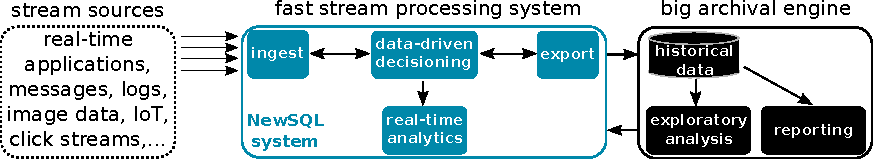
\includegraphics[width=.8\textwidth]{inputs/img/simple_newsql_data_stream}
  \caption{The emerging stream processing platforms for big data.}
  \label{fig:newsql_data_stream}
\end{figure}

\subsection{Anomaly detection using statistical learning}
\label{subsec:anomaly}

Statistical learning has been a widely used technique to predict performance anomalies in large-scale distributed systems~\cite{chandola2009anomaly}. It makes prediction by processing feature vector $\inpseq$ with a fixed
  number of dimensions $d$ ($\inpseq \in \inpspace \subset \Re^d$) from the input space $\mathcal{X}$. There are two main methods: \emph{supervised} and \emph{unsupervised learning}. 

The \emph{supervised learning method} couples each input with a $\rel$, a label, from the output space  $\mathcal{Y}$. To learn, we have $N$ pairs ($\inpseq,\rel$) drawn \emph{independent and identically distributed} (i.i.d.) from a fixed but unknown joint probability density function $\distspace$. This method searches for a function $\fscore$ : $\mathcal{X} \rightarrow \Re$  in a fixed function class $\fspace$ in the learning dataset. State-of-the-art algorithms, like \emph{random forests}~\cite{breiman2001random}, aim to find $\fscore^\star$ in $\fspace$ with the lowest empirical risk $\fscore^\star \in \argmin_{\fscore \in \fspace} \qm_{emp}(\fscore)$,
where $\qm_{emp}(\fscore) = \frac{1}{N} \sum_{i=1}^N \indic{\fscore(\inpseq) \neq \lab_i}$ is computed over the training set, and $\indic{.}$ is the indicator function which returns $1$ if the predicate $\{.\}$ is true and $0$ otherwise. Similarly, an \emph{unsupervised learning method} relies on $N$ unlabelled samples having probability density function $\distspacex$. Unlike supervised learning, predictions provide insights into how the data is organized or clustered.

Most of the anomaly detection approaches for distributed systems are based on a general-purpose, unsupervised learning method~\cite{gujrati2007meta,lan2010toward,guan2013adaptive}. However, prediction efficiency remains the main drawback of this method~\cite{love2002comparing}. Results in our previous work~\cite{silvestre2014anomaly} confirm that a supervised learning method overcomes an unsupervised one in cloud anomaly detection. In this work, we extend our supervised learning model as a component of Tejo to classify anomalous VMs in four different classes.
